\documentclass{article}
\usepackage{amsmath}
\usepackage{amsfonts}
\usepackage{tikz}
\usetikzlibrary{positioning, shapes.geometric}

\title{lec5/18}
\author{Dylan Tang}
\date{May 2026}

\begin{document}

\section{Encoder/Decoder Architecture}
\begin{itemize}
    \item An encoder/decoder architecture performs downsampling to a dense representation (encoding), then upsamples to predict the next token (decoding).
    \item Assumes that large, high/dimensional data can be represented by a lower dimensional, dense vector.
    \item The dense vector is also called an \textbf{embedding vector}.
        \begin{itemize}
                \item For GPT, the embedding vector is $\mathcal{R}^{768}$
        \end{itemize}
\end{itemize}


\subsection{Encoder/Decoder Funnel Structure}
\begin{center}
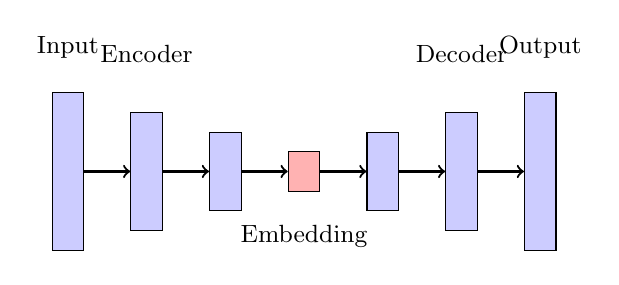
\begin{tikzpicture}[
    layer/.style={rectangle, draw, fill=blue!20, minimum width=0.4cm},
    arrow/.style={->, thick}
]

% Encoder (narrowing)
\node[layer, minimum height=2cm] (in) at (0, 0) {};
\node[layer, minimum height=1.5cm] (e1) at (1, 0) {};
\node[layer, minimum height=1cm] (e2) at (2, 0) {};
\node[layer, minimum height=0.5cm, fill=red!30] (bottleneck) at (3, 0) {};

% Decoder (expanding)
\node[layer, minimum height=1cm] (d1) at (4, 0) {};
\node[layer, minimum height=1.5cm] (d2) at (5, 0) {};
\node[layer, minimum height=2cm] (out) at (6, 0) {};

% Arrows
\draw[arrow] (in) -- (e1);
\draw[arrow] (e1) -- (e2);
\draw[arrow] (e2) -- (bottleneck);
\draw[arrow] (bottleneck) -- (d1);
\draw[arrow] (d1) -- (d2);
\draw[arrow] (d2) -- (out);

% Labels
\node[above=0.3cm of in] {\small Input};
\node[below=0.3cm of bottleneck] {\small Embedding};
\node[above=0.3cm of out] {\small Output};

\node[above=0.5cm of e1] {\small Encoder};
\node[above=0.5cm of d2] {\small Decoder};

\end{tikzpicture}
\end{center}

\subsection{Use Cases for Embedding Vectors}
\begin{itemize}
    \item Finding pages on the internet that are similar
        \begin{itemize}
            \item Convert each item to an embedding vector, compute degree of similarity with cosine similarity scores, edit distance, etc.
        \end{itemize}
    \item Compute new embedding vectors as weighted average of other embedding vectors
\end{itemize}

\section{Preventing Model Hallucinations}
There are several ways of preventing model hallucination:
\begin{itemize}
    \item Retrieval Augmented Generation (RAG): Model uses embedding vector to query database for precomputed embeddings that are accurate
\end{itemize}
\end{document}
